\documentclass[dvipdfmx,tikz]{standalone}
\usepackage{tikz,bm}
\begin{document}
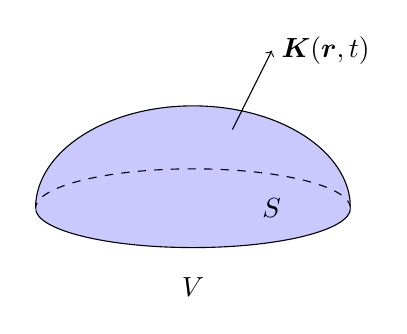
\begin{tikzpicture}
%\draw [help lines] (-2,-1) grid (2,2);
    \begin{scope}
        \clip (-2.1, 2) rectangle (2, 0);
        \draw [fill = blue!30!white!70!]circle [x radius = 2, y radius = 1.3];
        \draw [fill = blue!30!white!70!,dashed] circle [x radius = 2, y radius = 0.5];
    \end{scope}
    \begin{scope}
        \clip (-2, 0) rectangle (2, -0.7);
        \draw [fill = blue!30!white!70!]circle [x radius = 2, y radius = 0.5];
    \end{scope}
    \node at (0,-1) {$V$};
    \node at (1,0) {$S$};
    \draw[->] (0.5,1) -- (1,2) node[anchor = west] {$\bm{K}(\bm{r},t)$};
\end{tikzpicture}
\end{document}